\documentclass[tikz,border=8pt]{standalone}
% Shared look for every TikZ diagram. Load with % Shared look for every TikZ diagram. Load with % Shared look for every TikZ diagram. Load with \input{../../tools/tikz-style.tex}
\usepackage[T1]{fontenc}
\usepackage{lmodern}
\renewcommand{\sfdefault}{lmr}  % diagrams use the same serif as the text
\usetikzlibrary{arrows.meta, positioning, shapes.geometric, calc, fit, backgrounds}
\definecolor{cblue}{HTML}{4C78A8}
\definecolor{corange}{HTML}{F58518}
\definecolor{cgreen}{HTML}{54A24B}
\definecolor{cred}{HTML}{E45756}
\definecolor{cpurple}{HTML}{B279A2}
\definecolor{cgrey}{HTML}{6B6B6B}
\tikzset{
  every picture/.style={font=\sffamily, line width=1.2pt},
  box/.style={draw=#1, fill=#1!12, rounded corners=4pt, align=center, inner sep=7pt, minimum height=1.1cm},
  box/.default=cgrey,
  arrow/.style={-{Stealth[length=3mm]}, draw=cgrey, line width=1.4pt},
  title/.style={font=\sffamily\bfseries\Large},
  note/.style={font=\sffamily\small, text=cgrey, align=center},
}
\AtBeginDocument{\hyphenpenalty=10000 \exhyphenpenalty=10000}

\usepackage[T1]{fontenc}
\usepackage{lmodern}
\renewcommand{\sfdefault}{lmr}  % diagrams use the same serif as the text
\usetikzlibrary{arrows.meta, positioning, shapes.geometric, calc, fit, backgrounds}
\definecolor{cblue}{HTML}{4C78A8}
\definecolor{corange}{HTML}{F58518}
\definecolor{cgreen}{HTML}{54A24B}
\definecolor{cred}{HTML}{E45756}
\definecolor{cpurple}{HTML}{B279A2}
\definecolor{cgrey}{HTML}{6B6B6B}
\tikzset{
  every picture/.style={font=\sffamily, line width=1.2pt},
  box/.style={draw=#1, fill=#1!12, rounded corners=4pt, align=center, inner sep=7pt, minimum height=1.1cm},
  box/.default=cgrey,
  arrow/.style={-{Stealth[length=3mm]}, draw=cgrey, line width=1.4pt},
  title/.style={font=\sffamily\bfseries\Large},
  note/.style={font=\sffamily\small, text=cgrey, align=center},
}
\AtBeginDocument{\hyphenpenalty=10000 \exhyphenpenalty=10000}

\usepackage[T1]{fontenc}
\usepackage{lmodern}
\renewcommand{\sfdefault}{lmr}  % diagrams use the same serif as the text
\usetikzlibrary{arrows.meta, positioning, shapes.geometric, calc, fit, backgrounds}
\definecolor{cblue}{HTML}{4C78A8}
\definecolor{corange}{HTML}{F58518}
\definecolor{cgreen}{HTML}{54A24B}
\definecolor{cred}{HTML}{E45756}
\definecolor{cpurple}{HTML}{B279A2}
\definecolor{cgrey}{HTML}{6B6B6B}
\tikzset{
  every picture/.style={font=\sffamily, line width=1.2pt},
  box/.style={draw=#1, fill=#1!12, rounded corners=4pt, align=center, inner sep=7pt, minimum height=1.1cm},
  box/.default=cgrey,
  arrow/.style={-{Stealth[length=3mm]}, draw=cgrey, line width=1.4pt},
  title/.style={font=\sffamily\bfseries\Large},
  note/.style={font=\sffamily\small, text=cgrey, align=center},
}
\AtBeginDocument{\hyphenpenalty=10000 \exhyphenpenalty=10000}

\begin{document}
% Section 4: GPT-2's tokenizer on the Note's two example texts (Notebook). A common word is one token; a rare word
% is split into pieces. The leading space belongs to the token (drawn as an open box).
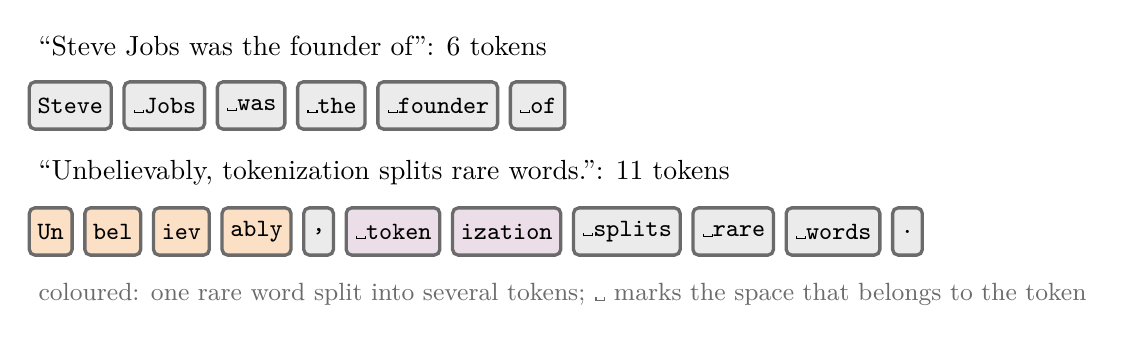
\begin{tikzpicture}[t/.style={draw=cgrey, fill=black!8, rounded corners=2pt, font=\ttfamily\small, inner sep=3pt, minimum height=0.6cm}]
  \node[font=\sffamily, anchor=west] at (0, 0.75) {``Steve Jobs was the founder of'': 6 tokens};
  \node[t, anchor=west] (a1) at (0, 0) {Steve};
  \foreach \w [count=\i from 2, remember=\i as \j (initially 1)] in {\textvisiblespace Jobs, \textvisiblespace was, \textvisiblespace the, \textvisiblespace founder, \textvisiblespace of}
    \node[t, anchor=west, right=0.12cm of a\j] (a\i) {\w};
  \node[font=\sffamily, anchor=west] at (0, -0.85) {``Unbelievably, tokenization splits rare words.'': 11 tokens};
  \node[t, anchor=west, fill=corange!25] (b1) at (0, -1.6) {Un};
  \foreach \w/\c [count=\i from 2, remember=\i as \j (initially 1)] in {bel/corange!25, iev/corange!25, ably/corange!25, {,}/black!8, \textvisiblespace token/cpurple!25, ization/cpurple!25, \textvisiblespace splits/black!8, \textvisiblespace rare/black!8, \textvisiblespace words/black!8, ./black!8}
    \node[t, anchor=west, right=0.12cm of b\j, fill=\c] (b\i) {\w};
  \node[note, anchor=west] at (0, -2.4) {coloured: one rare word split into several tokens; \textvisiblespace\ marks the space that belongs to the token};
\end{tikzpicture}
\end{document}
